% ============================================================================
%  Memoria — Predicción de cancelaciones de reservas hoteleras
%  Compilar:  make memo   (regenera figuras + compila con Tectonic; bootstrapea
%             el binario en .venv/bin la primera vez). Manual: tectonic memoria.tex
%  Las figuras del EDA se generan con:  python memoria/generar_figuras_eda.py
% ============================================================================
\documentclass[10pt,twocolumn,a4paper]{article}

\usepackage{fontspec}                       % XeTeX: UTF-8 nativo
\usepackage[spanish,es-noshorthands]{babel} % español sin shorthands conflictivos
\usepackage{geometry}
\geometry{a4paper,margin=1.9cm,columnsep=0.7cm}
\usepackage{graphicx}
\usepackage{float}   % opción [H]: ancla la figura EXACTAMENTE donde se declara
\usepackage{stfloats}  % permite figure* a pie de página ([b]) en doble columna
\usepackage{amsmath,amssymb}
\usepackage{booktabs}
\usepackage{array}
\usepackage{caption}
\usepackage{subcaption}
\usepackage{xcolor}
\usepackage{enumitem}
\usepackage{microtype}
\usepackage[hidelinks]{hyperref}
\usepackage{xurl}   % permite cortar URLs largas en cualquier carácter (evita overfull)
\usepackage{tikz}
\usetikzlibrary{positioning,arrows.meta,calc}

\graphicspath{{figuras/}{../outputs/}}

% --- estilo ---
\definecolor{azul}{HTML}{2c4f74}
\definecolor{gristexto}{HTML}{333333}
\captionsetup{font=small,labelfont={bf,color=azul},skip=4pt}
\setlist{nosep,leftmargin=1.2em}
\newcommand{\var}[1]{\texttt{#1}}           % identificadores de código

\usepackage{titlesec}
\titleformat{\section}{\large\bfseries\color{azul}}{\thesection.}{0.5em}{}
\titleformat{\subsection}{\normalsize\bfseries}{\thesubsection.}{0.5em}{}
\titlespacing*{\section}{0pt}{1.1ex}{0.6ex}
\titlespacing*{\subsection}{0pt}{0.9ex}{0.4ex}

\setlength{\parskip}{0.28em}
\setlength{\parindent}{0pt}

% --- Parámetros de flotantes: relajamos los límites conservadores de LaTeX para
%     que las figuras se coloquen lo más cerca posible de donde se mencionan
%     (más flotantes por página, menos texto mínimo reservado).
\setcounter{topnumber}{3}
\setcounter{bottomnumber}{3}
\setcounter{totalnumber}{6}
\setcounter{dbltopnumber}{3}
\renewcommand{\topfraction}{0.92}
\renewcommand{\bottomfraction}{0.9}
\renewcommand{\textfraction}{0.06}
\renewcommand{\floatpagefraction}{0.7}
\renewcommand{\dbltopfraction}{0.92}
\renewcommand{\dblfloatpagefraction}{0.7}

% ============================================================================
\begin{document}

% ---- Bloque de cabecera a UNA columna (ancho completo) ---------------------
\twocolumn[{%
\begin{center}
  {\LARGE\bfseries\color{azul} Predicción de cancelaciones de reservas hoteleras}\\[0.4em]
  {\large Memoria del Proyecto Final de Módulo}\\[0.3em]
  {\normalsize Máster en IA, Cloud Computing y DevOps\,\textbullet\, Módulo de Machine Learning y Deep Learning}\\[0.7em]
  {\normalsize Manuel Pérez Martínez\quad Joaquín Castro Salas}\\[0.15em]
  {\small\ttfamily manugijon@gmail.com\quad jcastrosalas03@gmail.com}\\[0.25em]
  {\small\ttfamily\url{https://github.com/manupm87/pontia-ml}}
\end{center}
\vspace{0.4em}

\begin{center}
  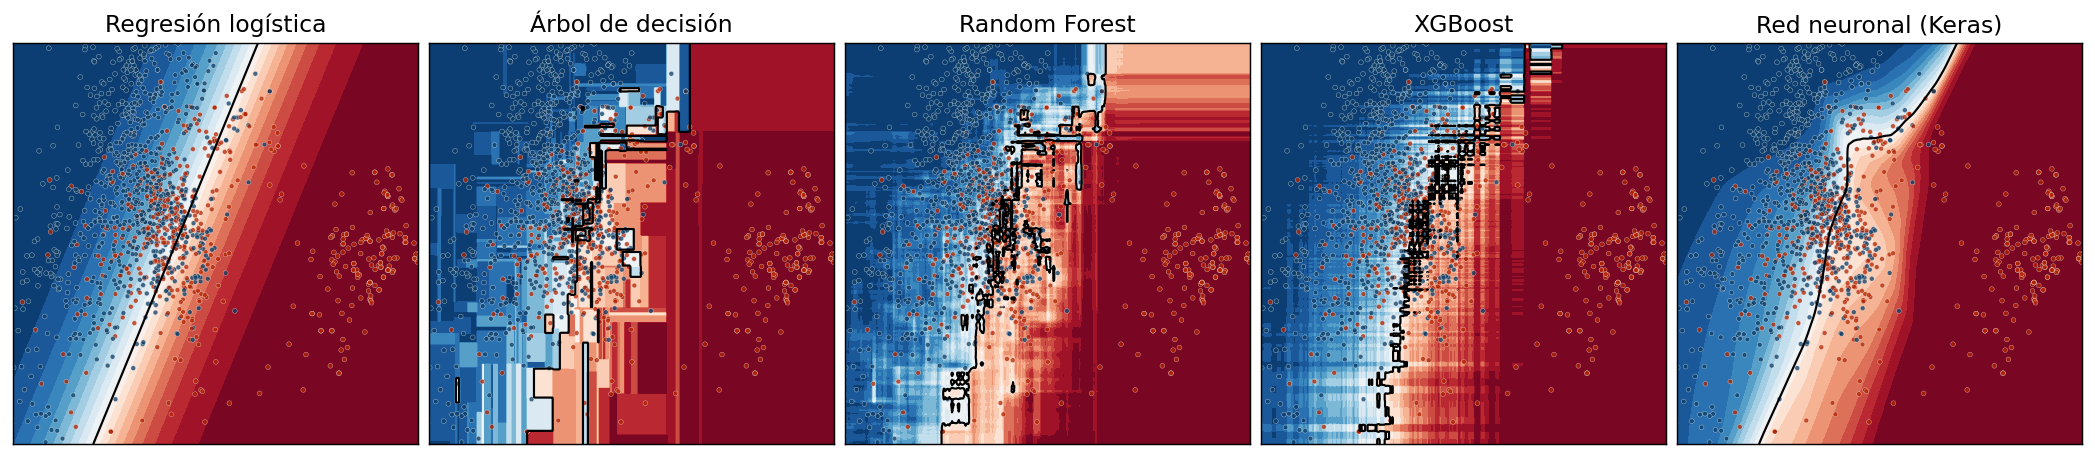
\includegraphics[width=0.99\textwidth]{decision_regions_strip.png}\\[0.3em]
  {\small\captionof{figure}{Regiones de decisión aprendidas por los cinco modelos sobre
  el mismo plano 2D supervisado (PLS): el color es la probabilidad estimada de
  cancelación (azul$\to$rojo) y los puntos, reservas reales del conjunto de prueba.
  Anticipa visualmente la comparativa de la Sección~4.}}
\end{center}
\vspace{0.8em}

\noindent\textbf{\color{azul}Resumen.}\;
Las cancelaciones tardías de reservas vacían habitaciones difíciles de revender y
distorsionan la previsión de ocupación del hotel. Este trabajo aborda la
predicción de la cancelación de una reserva (\var{is\_canceled}) como un problema de
\textbf{clasificación binaria} sobre $\sim$119\,000 reservas y 31 características.
Partiendo de un análisis exploratorio que detecta y corrige varias fugas de
información, se diseña un \emph{pipeline} de preprocesado reproducible (derivación de
variables, reducción supervisada de cardinalidad, imputación, estandarización y
codificación \emph{one-hot}) y se comparan cinco familias de modelos. El ganador,
\textbf{XGBoost}, alcanza un \textbf{ROC-AUC de 0.9529} sobre un conjunto de prueba
independiente. El modelo se sirve mediante una API REST (FastAPI) y se muestra en una
interfaz web (Streamlit) que predice e interpreta cada reserva con SHAP.
\vspace{0.6em}

\noindent\textbf{\color{azul}Roles y reparto del trabajo.}\;
El proyecto se ha desarrollado de forma plenamente colaborativa: ambos integrantes
participaron en todas las fases del trabajo ---análisis exploratorio, diseño del
\emph{pipeline}, entrenamiento y comparación de modelos, productivización (API y UI)
y documentación---. El método de trabajo fue principalmente el \emph{pair
programming}: las decisiones técnicas se tomaron y se pusieron en común de forma
conjunta en sesiones compartidas, de modo que ambos asumen por igual la
responsabilidad sobre el conjunto del sistema.
\vspace{1.2em}
}]

% ============================================================================
\section{Justificación del problema}

Las \textbf{cancelaciones de reservas} son uno de los principales problemas
económicos del sector hotelero. Una cancelación, sobre todo si llega con poca
antelación, deja una habitación vacía que rara vez vuelve a venderse: se pierde el
ingreso de esa noche y, con él, parte del margen del establecimiento. El daño va más
allá del ingreso directo, porque las cancelaciones \textbf{distorsionan la previsión
de ocupación} sobre la que se planifican el personal, los aprovisionamientos y los
precios, complicando la gestión diaria del hotel.

Para defenderse, los hoteles recurren a prácticas como el \emph{overbooking}
(aceptar más reservas que plazas contando con que algunas se cancelarán), la
exigencia de depósitos o las campañas de retención. Todas comparten un requisito:
solo son seguras y rentables si el hotel puede \textbf{anticipar qué reservas tienen
más riesgo} de cancelarse. Una estimación fiable de ese riesgo permite actuar de
forma selectiva ---sobrevender en la medida justa, pedir garantías a las reservas
dudosas o intervenir antes de que el cliente cancele--- y proteger así los ingresos y
la calidad del servicio.

Anticipar las cancelaciones es, por tanto, un problema con un retorno claro y directo
para el negocio, lo que justifica el esfuerzo de construir un sistema que las prediga.

Formalmente, representamos la cancelación como una variable aleatoria binaria
$Y \in \{0,1\}$ ($Y=1$ si la reserva se cancela). El sistema estima la probabilidad
condicionada $\hat{p}(\mathbf{x}) = P(Y=1 \mid \mathbf{x})$ a partir del vector de
características $\mathbf{x} \in \mathbb{R}^{D}$, y la decisión final se obtiene aplicando
un umbral $\tau$:
\begin{equation}
\hat{Y} =
\begin{cases}
1 & \text{si } \hat{p}(\mathbf{x}) \geq \tau, \\
0 & \text{si } \hat{p}(\mathbf{x}) < \tau,
\end{cases}
\end{equation}
donde $\tau$ puede ajustarse según la matriz de costes del hotel, ponderando el coste de
un falso negativo (habitación vacía) frente al de un falso positivo (compensación por
\emph{overbooking}).

% ============================================================================
\section{Análisis exploratorio de datos}

El EDA es la fase en la que exploramos los datos con tablas y gráficos \emph{antes de
modelar}, para tomar decisiones con fundamento. Cada hallazgo de esta sección se
tradujo en una decisión de diseño concreta del \emph{pipeline}.

\subsection{La clase objetivo está desbalanceada}

Alrededor del \textbf{37\,\%} de las reservas se cancelan frente a un 63\,\% que no
(Figura~\ref{fig:desbalance}). Es un desbalance moderado.
\textit{Decisión:} usar una \textbf{partición estratificada} (preservar ese 37\,\%
en entrenamiento y prueba) y elegir el \textbf{ROC-AUC} como métrica principal en
lugar de la \emph{accuracy}, que premiaría a un clasificador trivial.

\begin{figure}[tb]
  \centering
  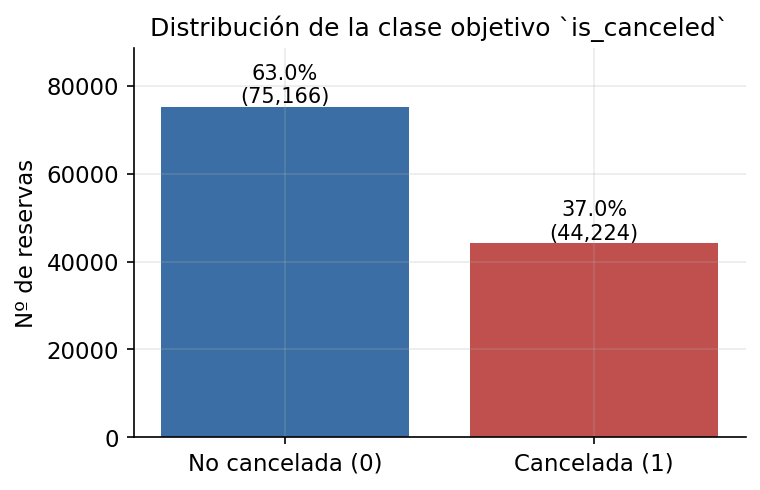
\includegraphics[width=\columnwidth]{eda_desbalance_clase.png}
  \caption{Reparto de la clase objetivo. El desbalance ($\sim$37\,/\,63) motiva la
  estratificación y el uso de ROC-AUC.}
  \label{fig:desbalance}
\end{figure}

\subsection{Columnas que ``hacen trampa'' (fuga de información)}

La \textbf{fuga de información} (\emph{data leakage}) ocurre cuando el modelo usa, sin
querer, datos que revelan la respuesta o que no existirían en el momento de predecir.

\var{reservation\_status} vale \var{Canceled}/\var{No-Show} \emph{exactamente} cuando
\var{is\_canceled}\,$=1$, y junto con \var{reservation\_status\_date} describe lo que
ocurrió \emph{después} de decidir la cancelación. \textit{Decisión:} eliminar ambas
columnas; de lo contrario el modelo ``vería la respuesta'' y obtendría un acierto
del $\sim$100\,\% engañoso e inútil.

Más sutil es \var{required\_car\_parking\_spaces}
(Figura~\ref{fig:parking}): ninguna reserva con plaza de parking se cancela
(0\,\%), pero esa relación es \emph{determinista} precisamente porque el dato
\textbf{solo se conoce en el \emph{check-in}}, cuando el cliente ya se ha presentado
y, por tanto, no ha cancelado. El 0\,\% se mantiene incluso restringiendo a las
reservas cancelables (\var{deposit\_type} = \var{No Deposit}), lo que descarta que
sea una mera correlación con el depósito. \textit{Decisión:} \textbf{eliminarla} del
modelo: en el momento de puntuar una reserva futura ese valor no existe. Era la
principal causa del optimismo de versiones anteriores.

\begin{figure}[tb]
  \centering
  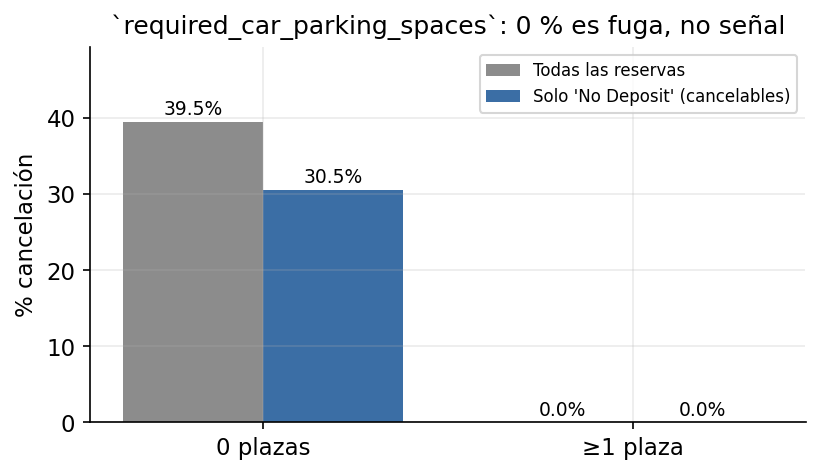
\includegraphics[width=\columnwidth]{eda_fuga_parking.png}
  \caption{\var{required\_car\_parking\_spaces}: el 0\,\% de cancelación con plaza
  asignada persiste dentro de las reservas cancelables, revelando una fuga de
  \emph{check-in}, no un predictor.}
  \label{fig:parking}
\end{figure}

La misma lógica descarta \var{assigned\_room\_type}, el tipo de habitación
\textbf{finalmente asignado}: solo se conoce en el \emph{check-in}. Cuando la
habitación asignada \textbf{difiere} de la reservada la cancelación cae al
5.4\,\% (frente al 41.6\,\% cuando coinciden), porque reasignar habitación
implica que el cliente se presentó. Se elimina; \var{reserved\_room\_type} ---la que
el cliente elige al reservar--- sí se conserva.

También se descarta \var{arrival\_date\_year}: apenas discrimina (la tasa es casi
idéntica los tres años), no generaliza a años futuros no vistos y va confundido con la
estación (correlación $-0.54$ con la semana del año, porque el dataset cubre años
parciales). La señal estacional ya la recogen \var{arrival\_date\_month} y
\var{week\_number}, que sí se repiten cada año.

\subsection{Valores ausentes}

Cuatro columnas presentan huecos (Figura~\ref{fig:nulos}). En lugar de descartarlas,
se tratan según su naturaleza: \var{company} ($\sim$94\,\% vacía) y \var{agent} se
conservan como categorías (el hueco pasa a una etiqueta propia), \var{country} se
imputa con una constante y \var{children} con 0. La imputación se aprende
\emph{solo en entrenamiento} para no filtrar información del test.

\begin{figure}[tb]
  \centering
  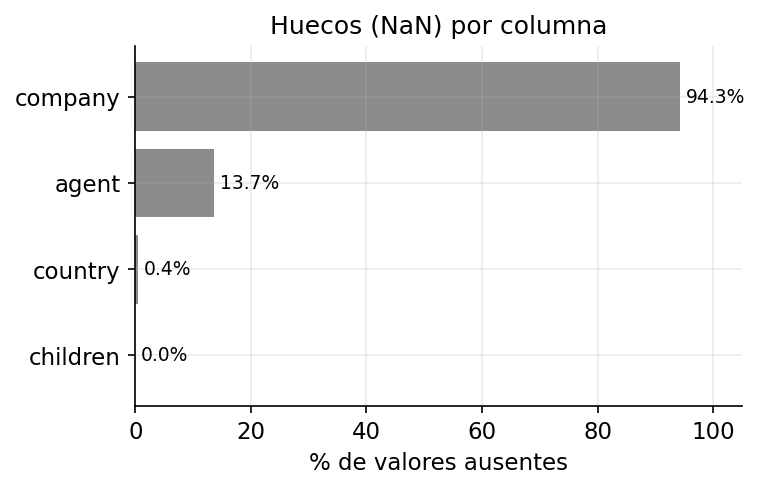
\includegraphics[width=\columnwidth]{eda_valores_ausentes.png}
  \caption{Porcentaje de valores ausentes por columna. \var{company} está casi
  totalmente vacía, pero su ausencia es informativa.}
  \label{fig:nulos}
\end{figure}

\subsection{La ausencia es señal, no ruido}

Que una reserva no tenga \var{company} o \var{agent} asignado no es un simple hueco:
es una señal con valor predictivo (Figura~\ref{fig:ausencia}). Las reservas
\textbf{con} empresa cancelan mucho menos que las que no la tienen; con \var{agent}
la señal va en sentido contrario. \textit{Decisión:} derivar dos indicadores binarios
\var{has\_company} y \var{has\_agent} que capturan explícitamente esa diferencia, en
vez de descartar las columnas.

\begin{figure}[tb]
  \centering
  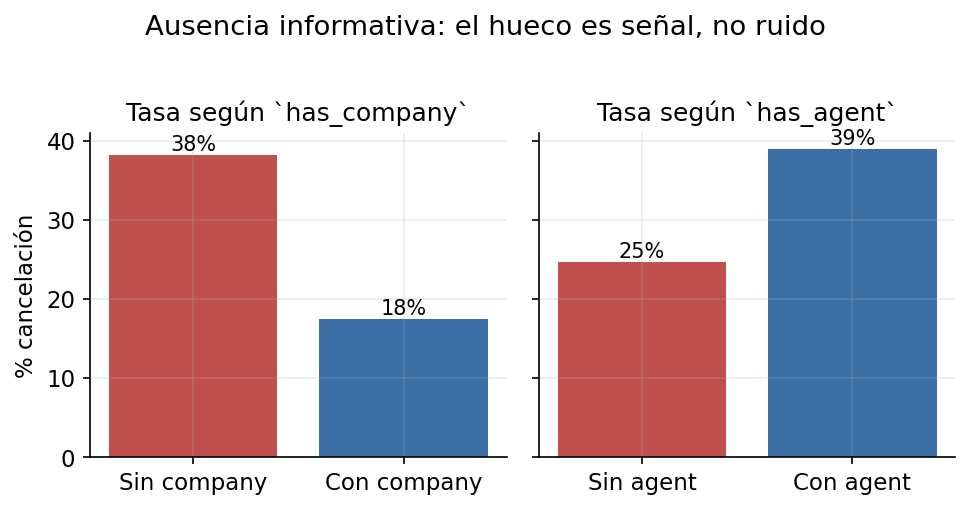
\includegraphics[width=\columnwidth]{eda_ausencia_informativa.png}
  \caption{Tasa de cancelación según la presencia/ausencia de \var{company} y
  \var{agent}. La ausencia discrimina, lo que justifica las variables derivadas
  \var{has\_company}/\var{has\_agent}.}
  \label{fig:ausencia}
\end{figure}

\subsection{Variables numéricas}

\var{lead\_time} (días de antelación) es la numérica más relacionada con la
cancelación: a más antelación, mayor probabilidad de cancelar, de forma casi
monótona por tramos (Figura~\ref{fig:leadtime}). \var{total\_of\_special\_requests}
se relaciona a la inversa (clientes más comprometidos cancelan menos). Como las
variables conviven en escalas muy distintas, se aplica \textbf{estandarización}
(media 0, desviación 1) para que ningún rango domine artificialmente.
Esta transformación \textbf{no perjudica a ningún modelo}: los basados en árboles
(Random Forest y XGBoost, el ganador) son insensibles a la escala ---deciden por cortes
y el orden de los valores no cambia---, mientras que la regresión logística y la red
neuronal sí se benefician de ella (convergen mejor y sus coeficientes son comparables).
Por eso, aunque matemáticamente algunas variables no la necesiten, la aplicamos de forma
\textbf{global}: simplifica el \emph{pipeline} y no introduce ningún efecto negativo.

\begin{figure}[tb]
  \centering
  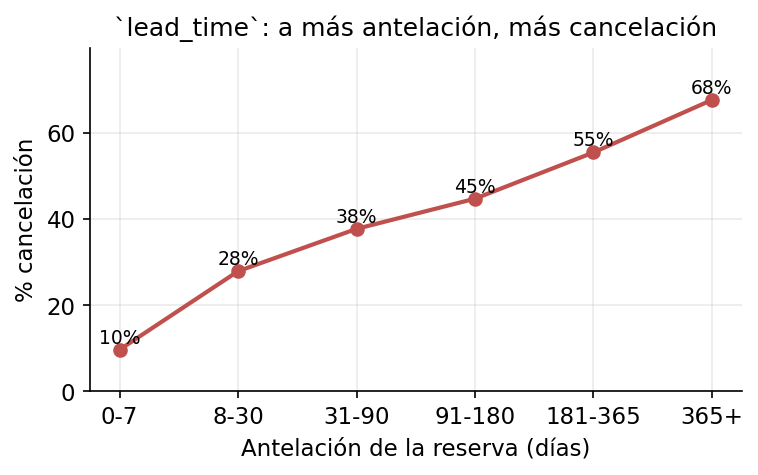
\includegraphics[width=\columnwidth]{eda_lead_time.png}
  \caption{Tasa de cancelación por tramos de \var{lead\_time}: relación creciente y
  casi monótona, la señal numérica más fuerte.}
  \label{fig:leadtime}
\end{figure}

\subsection{Variables categóricas y codificación}

\var{deposit\_type} = \var{Non Refund} (depósito no reembolsable) tiene una tasa de
cancelación \textbf{cercana al 99\,\%} (Figura~\ref{fig:deposit}): la variable más
predictiva del conjunto. Las categóricas se transforman a números mediante
codificación \textbf{\emph{one-hot}} (\var{OneHotEncoder}), una columna binaria por
categoría.

\begin{figure}[tb]
  \centering
  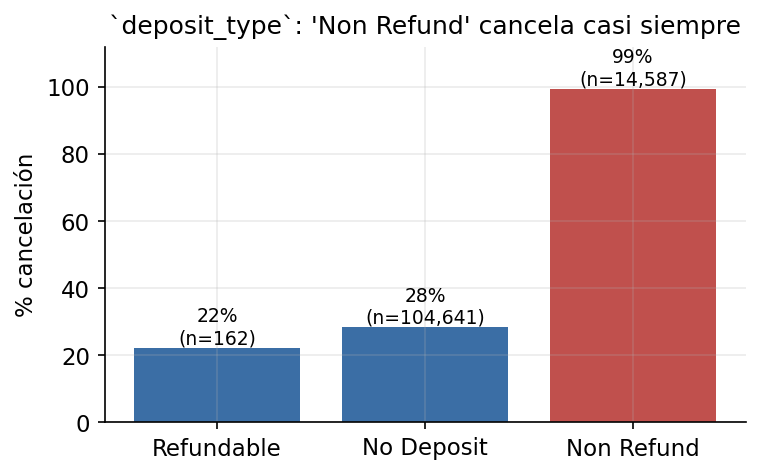
\includegraphics[width=\columnwidth]{eda_deposit_type.png}
  \caption{\var{deposit\_type}: el depósito no reembolsable casi garantiza la
  cancelación. Señal categórica dominante.}
  \label{fig:deposit}
\end{figure}

El problema es que \var{country} (177 países), \var{agent} (333 agencias) y
\var{company} (352) tienen \textbf{altísima cardinalidad}
(Figura~\ref{fig:cardinalidad}): un \emph{one-hot} directo crearía cientos de columnas
casi vacías, disparando la dimensionalidad y el sobreajuste. \textit{Decisión:}
aplicar una \textbf{reducción supervisada de cardinalidad} \emph{antes} del
\emph{one-hot}, implementada como un \textbf{transformador propio}
(\texttt{RareCategoryGrouper}, ya que \texttt{scikit-learn} no incluye ninguno que
agrupe categorías según el \emph{target}). Se conservan las categorías con soporte
suficiente ($n \geq 100$) y tasa de cancelación \textbf{extrema en cualquiera de los dos
sentidos} (muy alta o muy baja, con umbral adaptativo por variable: $>0.6$ o $<0.3$ de la
tasa máxima de esa columna); el resto se agrupa en \var{Otros}. La selección usa el
objetivo, así que se aprende \textbf{solo con el \emph{train}} y se reaplica idéntica en
test e inferencia (sin fuga). Lo verificamos entrenando los 5 modelos con y sin la
reducción: pasamos de \textbf{902 a 144 columnas} sin coste para \textbf{XGBoost}
(ROC-AUC $0.9529$ vs.\ $0.9573$, dentro del ruido) y con mejora para \textbf{Random
Forest} ($0.9363$ vs.\ $0.9221$). Así se preserva la señal de las categorías relevantes
sin pagar el coste dimensional. La Figura~\ref{fig:keepcats} muestra, en sus tres
paneles, \emph{qué} categorías sobreviven en cada variable, ordenadas por tasa de
cancelación: en rojo las de \textbf{alto riesgo} (tasa $>0.6$ del máximo de la columna)
y en azul las \textbf{muy fiables} ($<0.3$ del máximo). El resto, sin señal extrema, se
agrupa en \var{Otros}.

\begin{figure}[tb]
  \centering
  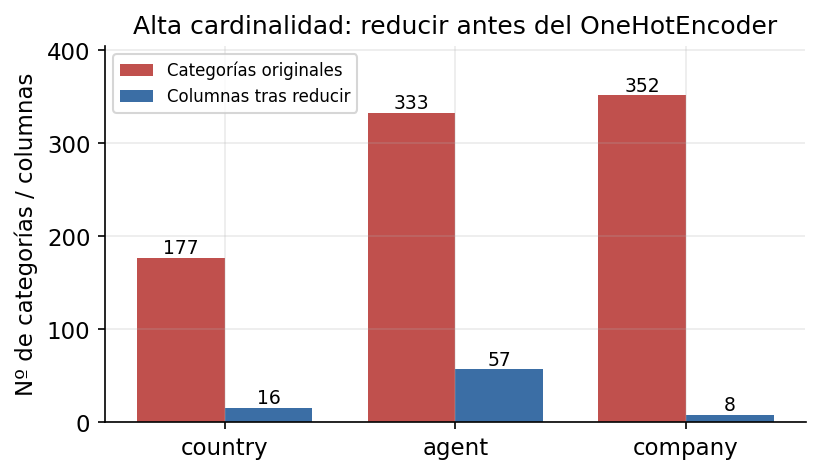
\includegraphics[width=\columnwidth]{eda_cardinalidad.png}
  \caption{Reducción supervisada de cardinalidad: de cientos de categorías a unas
  pocas columnas con señal, paso previo al \var{OneHotEncoder}.}
  \label{fig:cardinalidad}
\end{figure}

\begin{figure}[tb]
  \centering
  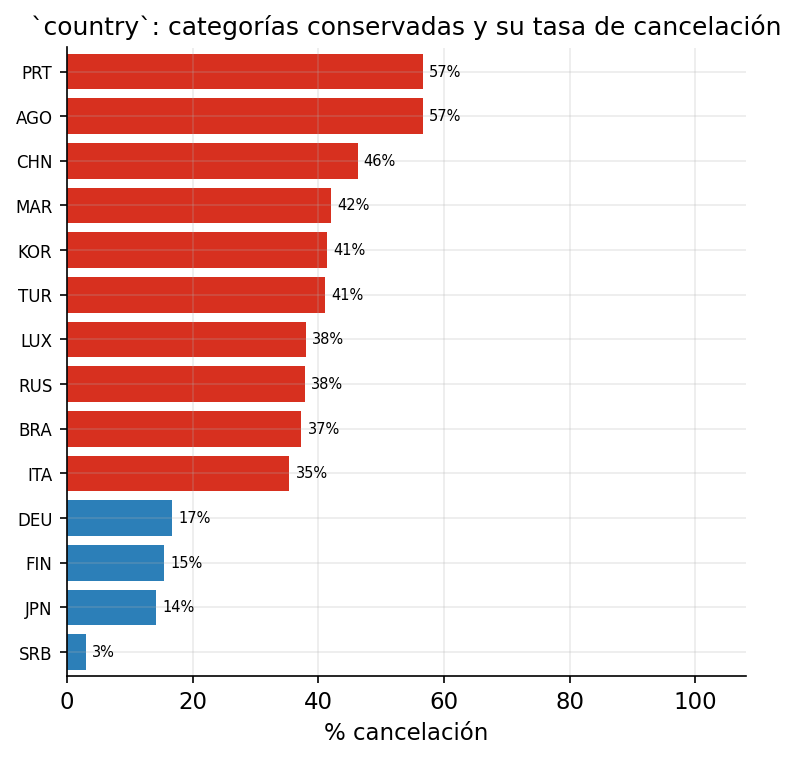
\includegraphics[width=0.80\columnwidth]{eda_keep_country.png}\\[4pt]
  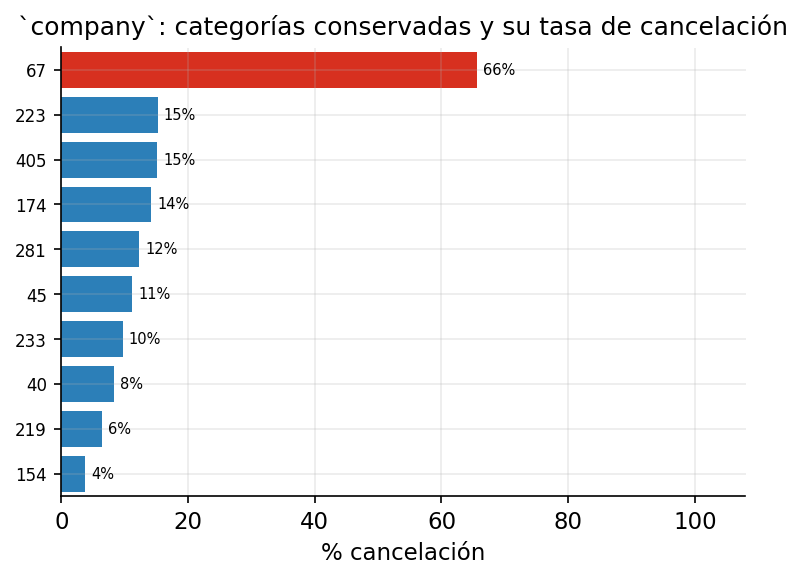
\includegraphics[width=0.80\columnwidth]{eda_keep_company.png}\\[4pt]
  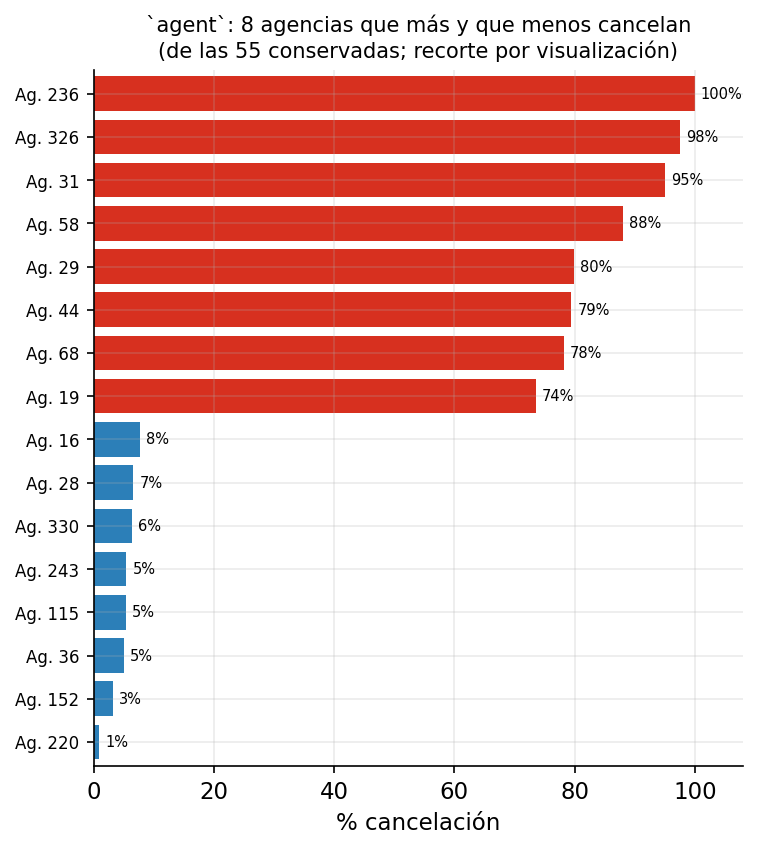
\includegraphics[width=0.80\columnwidth]{eda_keep_agent.png}
  \caption{Categorías conservadas por la reducción supervisada en las tres variables de
  alta cardinalidad, una bajo otra por tratar lo mismo: \var{country} (14 conservadas;
  Portugal y Angola, alto riesgo), \var{company} (10) y \var{agent}. Ordenadas por tasa
  de cancelación ---en rojo el alto riesgo, en azul las muy fiables; el resto va a
  \var{Otros}---. En \var{agent} se muestran solo las 8 que más y las 8 que menos
  cancelan (de las $\sim$55 conservadas), por legibilidad.}
  \label{fig:keepcats}
\end{figure}

Por último, se sanea el conjunto eliminando registros claramente erróneos:
$\sim$180 reservas sin ningún huésped (\var{adults}+\var{children}+\var{babies}
$=0$) y dos \emph{outliers} flagrantes en la tarifa diaria \var{adr} ---un valor
\textbf{negativo} ($-6.4$) y otro \textbf{desorbitado} ($5400$)--- que solo pueden ser
errores de captura.

% ============================================================================
\section{Diseño del sistema}

El sistema no se construyó de una vez, sino siguiendo un \textbf{arco de desarrollo}
en tres etapas que va de la exploración libre a un servicio en producción. La
progresión es deliberada: cada etapa valida sus decisiones antes de comprometerlas en
la siguiente.

\subsection{Etapa 1 --- Exploración con cuadernos}

La fase exploratoria se realizó en \emph{notebooks} autónomos, donde se analizaron los
datos y se prototiparon a mano las reglas de preparación y los primeros modelos. Es el
terreno para equivocarse barato: probar codificaciones, detectar y descartar variables
con fuga, medir el efecto del balanceo de clases, etc. De aquí salieron ya validadas
todas las decisiones del EDA de la sección anterior.

\subsection{Etapa 2 --- Generalización en un \emph{pipeline}}

Lo aprendido se consolidó en un \emph{pipeline} de preprocesado reproducible que
encadena, como pasos sucesivos, la derivación de variables informativas (entre ellas
\var{has\_company}/\var{has\_agent}), la reducción supervisada de cardinalidad de las
categóricas, la imputación de huecos, la estandarización de las numéricas y la
codificación \emph{one-hot}. La clave metodológica es que el preprocesado se
\textbf{ajusta únicamente con los datos de entrenamiento} y se guarda \emph{junto al
modelo}: así se evita cualquier fuga hacia el conjunto de prueba y se garantiza que la
inferencia replica exactamente el entrenamiento. Sobre ese preprocesado común se
entrenan y comparan, en igualdad de condiciones, \textbf{cinco familias de modelos}
---regresión logística (línea base), árbol de decisión, Random Forest, XGBoost y una
red neuronal multicapa con \textbf{Keras/TensorFlow} (densas $64\!\to\!32\!\to\!16$ con
\emph{dropout} y salida sigmoide)---, con sus hiperparámetros optimizados por validación
cruzada. La Figura~\ref{fig:pipeline} resume este flujo de extremo a extremo.

\begin{figure}[tb]
  \centering
  \resizebox{\columnwidth}{!}{%
  \begin{tikzpicture}[
    >={Latex[length=2.2mm]},
    stage/.style={draw, rounded corners=2pt, align=center, font=\small\sffamily,
                  minimum height=8mm, text width=42mm, line width=0.5pt},
    node distance=4.5mm,
  ]
    \node[stage, fill=orange!12] (d) {\textbf{Datos crudos}\\[1pt]\scriptsize $\sim$119\,k reservas};
    \node[stage, fill=blue!10, below=of d]   (p) {\textbf{Preprocesado}\\[1pt]\scriptsize derivar · reducir cardinalidad\\\scriptsize imputar · escalar · one-hot};
    \node[stage, fill=violet!10, below=of p] (t) {\textbf{Entrenamiento}\\[1pt]\scriptsize 5 modelos (tuning por CV)};
    \node[stage, fill=violet!10, below=of t] (e) {\textbf{Evaluación}\\[1pt]\scriptsize ROC-AUC · selección del mejor};
    \node[stage, fill=teal!14, below=of e]   (r) {\textbf{Registro}\\[1pt]\scriptsize modelo persistido + MLflow};
    \node[stage, fill=green!14, below=of r]  (i) {\textbf{Inferencia}\\[1pt]\scriptsize API + interfaz};
    \draw[->] (d) -- (p);
    \draw[->] (p) -- (t);
    \draw[->] (t) -- (e);
    \draw[->] (e) -- (r);
    \draw[->] (r) -- (i);
    % anotación lateral: el preprocesado, ajustado en train, viaja hasta la inferencia
    \draw[->, dashed, gray] (p.east) -- ++(7mm,0) |- (i.east);
    \node[font=\scriptsize\itshape, text=black!60, align=left, text width=23mm, right=10mm of e]
      {el preprocesado (ajustado solo en \emph{train}) viaja con el modelo};
  \end{tikzpicture}%
  }
  \caption{El \emph{pipeline} de ML de extremo a extremo (flujo vertical):
  preprocesado, entrenamiento y evaluación de los modelos, registro del ganador e
  inferencia. El preprocesado se aprende del entrenamiento y se persiste junto al modelo,
  de modo que predecir reproduce exactamente las transformaciones del entrenamiento.}
  \label{fig:pipeline}
\end{figure}

\paragraph{¿Qué es la validación cruzada?} En lugar de fiar la elección de
hiperparámetros a una única partición, la \emph{validación cruzada} ($k$\emph{-fold})
divide el entrenamiento en $k$ bloques: entrena con $k-1$ y mide en el bloque restante,
rotando hasta que cada bloque ha servido una vez de validación. El promedio de las $k$
medidas es una estimación \textbf{más estable y menos optimista} del rendimiento, y evita
ajustar los hiperparámetros al azar de un único reparto. La configuración finalmente
elegida es la que mejor puntúa en ese promedio.

\subsection{Etapa 3 --- Productivización}

Finalmente, el modelo ganador se lleva a producción. El artefacto se persiste y se
\textbf{versiona en un registro de modelos} (MLflow), el código y el modelo viven en
un repositorio Git, y dos servicios desplegados de forma continua exponen el sistema
al usuario: una \textbf{API REST} (FastAPI) que sirve las predicciones y una
\textbf{interfaz web} (Streamlit) que permite explorar los resultados y predecir
reservas concretas consumiendo esa API. La Figura~\ref{fig:arquitectura} resume la
arquitectura en cuatro planos ---experimentación, trazabilidad, repositorio y
servicio--- que pueden evolucionar de forma independiente: una nueva iteración de
modelado solo afecta a los dos primeros, y un cambio de interfaz, solo al último.

\begin{figure*}[tb]
  \centering
  \resizebox{\textwidth}{!}{%
  \begin{tikzpicture}[
    >={Latex[length=2.6mm]},
    box/.style={draw, rounded corners=2pt, align=center, font=\small\sffamily,
                minimum height=13mm, text width=22mm, line width=0.5pt},
    node distance=6mm and 8mm,
  ]
    \node[box, fill=orange!12] (data) {\textbf{Datos}\\[1pt]\scriptsize hotel bookings};
    \node[box, fill=blue!10, right=of data] (exp) {\textbf{Experimentación}\\[1pt]\scriptsize entrenamiento\\\scriptsize + tuning (local)};
    \node[box, fill=teal!14, right=of exp]  (pkl) {\textbf{Modelo}\\[1pt]\scriptsize XGBoost\\\scriptsize persistido};
    \node[box, fill=teal!10, right=of pkl]  (repo) {\textbf{Repositorio}\\[1pt]\scriptsize GitHub};
    \node[box, fill=red!10, right=of repo]  (svc) {\textbf{Servicio}\\[1pt]\scriptsize FastAPI (Render)\\\scriptsize Streamlit (Cloud)};
    \node[box, fill=green!14, right=of svc] (user) {\textbf{Usuario}\\[1pt]\scriptsize navegador};
    \node[box, fill=violet!10, above=10mm of pkl] (mlf) {\textbf{MLflow}\,·\,DagsHub\\[1pt]\scriptsize Experiments\\\scriptsize Model Registry};
    \draw[->] (data) -- (exp);
    \draw[->] (exp) -- (pkl);
    \draw[->] (pkl) -- (repo);
    \draw[->] (repo) -- (svc);
    \draw[<->] (svc) -- (user);
    \draw[->] (exp) -- (mlf);
    \draw[->, dashed, gray] (mlf) -- (svc);
  \end{tikzpicture}%
  }
  \caption{Arquitectura en cuatro planos. El dato alimenta la experimentación local,
  que emite un modelo versionado (MLflow/DagsHub) y un artefacto en el repositorio; de
  ahí, el despliegue continuo publica la API y la interfaz que consume el usuario. La
  flecha discontinua indica que el servicio puede cargar el modelo directamente desde
  el registro.}
  \label{fig:arquitectura}
\end{figure*}

\paragraph{Despliegue público.} El sistema está accesible en línea (servicios en
\emph{tier} gratuito, pueden tardar unos segundos en activarse tras inactividad):
\begin{itemize}
  \item \textbf{Interfaz web} (Streamlit): {\small\url{https://ml-hotel-cancellations-manupm87.streamlit.app}}
  \item \textbf{API REST} (FastAPI, Swagger): {\small\url{https://pontia-api-fi8t.onrender.com/docs}}
  \item \textbf{Experimentos y registro de modelos} (MLflow en DagsHub): {\small\url{https://dagshub.com/manupm87/pontia-ml.mlflow}}
\end{itemize}

\subsection{Interpretabilidad}

Un sistema que decide sobre el negocio debe poder \textbf{explicar} sus decisiones, no
solo acertar. Por eso el diseño incorpora interpretabilidad con \textbf{SHAP}, una
técnica que reparte cada predicción entre las variables, indicando cuánto empuja cada
una hacia ``cancela'' o ``no cancela'', a nivel \textbf{global} (qué pesa en general)
y \textbf{local} (por qué \emph{esa} reserva concreta).

\paragraph{A nivel global.} El resumen SHAP (Figura~\ref{fig:shap}) lo encabeza
\var{deposit\_type}~=~\var{Non Refund}, seguido del país (Portugal,
\var{country\_PRT}), el \var{lead\_time}, el total de peticiones especiales, el segmento
de mercado (\var{Online TA}) y las cancelaciones previas. Aparece también
\var{agent\_Otros}, lo que confirma que el grupo de agencias condensado por la reducción
de cardinalidad sí aporta señal. La importancia interna del Random Forest
(Figura~\ref{fig:fimp}) ordena las variables de forma muy parecida: que dos familias
de modelos distintas coincidan en lo que importa refuerza que el sistema aprende
patrones reales, no artefactos de un algoritmo concreto.

\begin{figure*}[tb]
  \centering
  \begin{subfigure}[t]{0.46\textwidth}
    \centering
    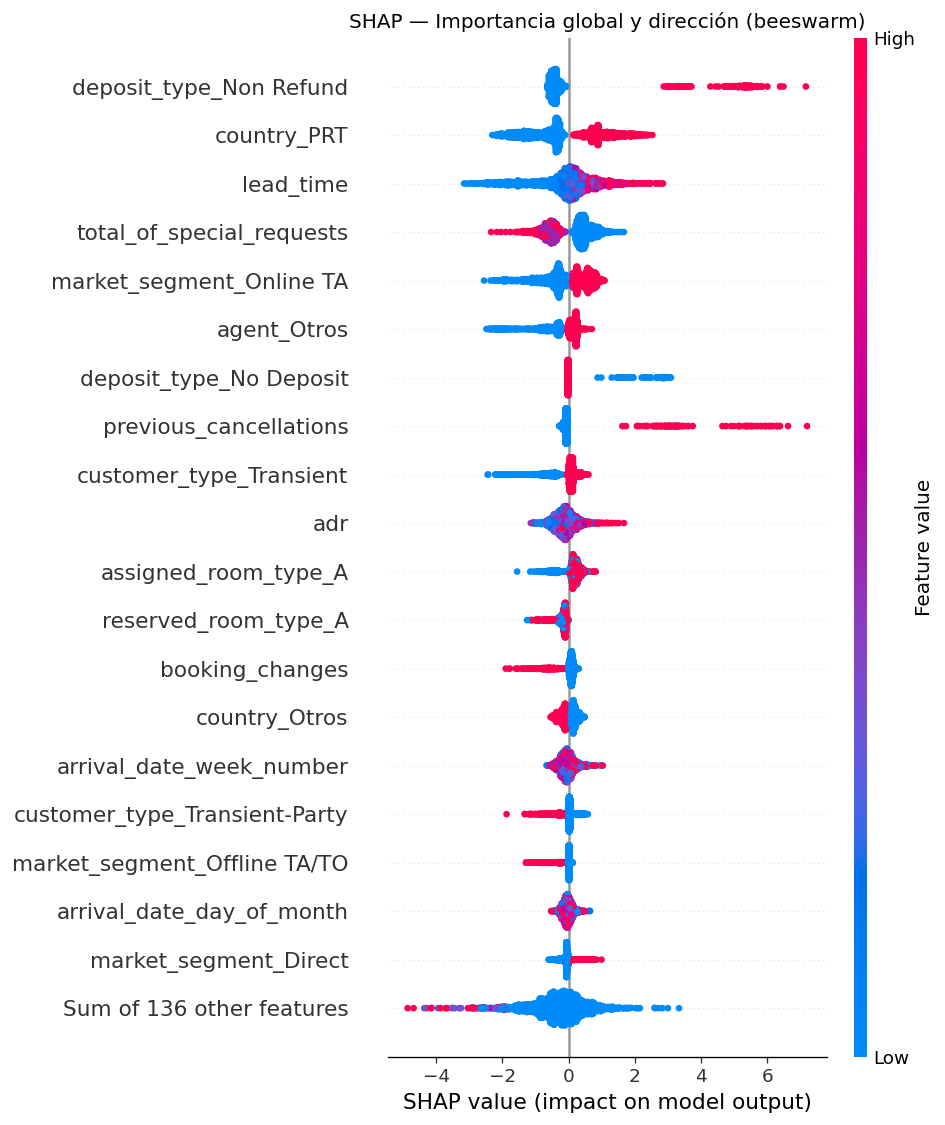
\includegraphics[width=\linewidth]{shap_summary_beeswarm.png}
    \caption{Resumen SHAP global (\emph{beeswarm}) del modelo ganador: aporte y dirección
    de cada variable. Confirma los hallazgos del EDA.}
    \label{fig:shap}
  \end{subfigure}\hfill
  \begin{subfigure}[t]{0.46\textwidth}
    \centering
    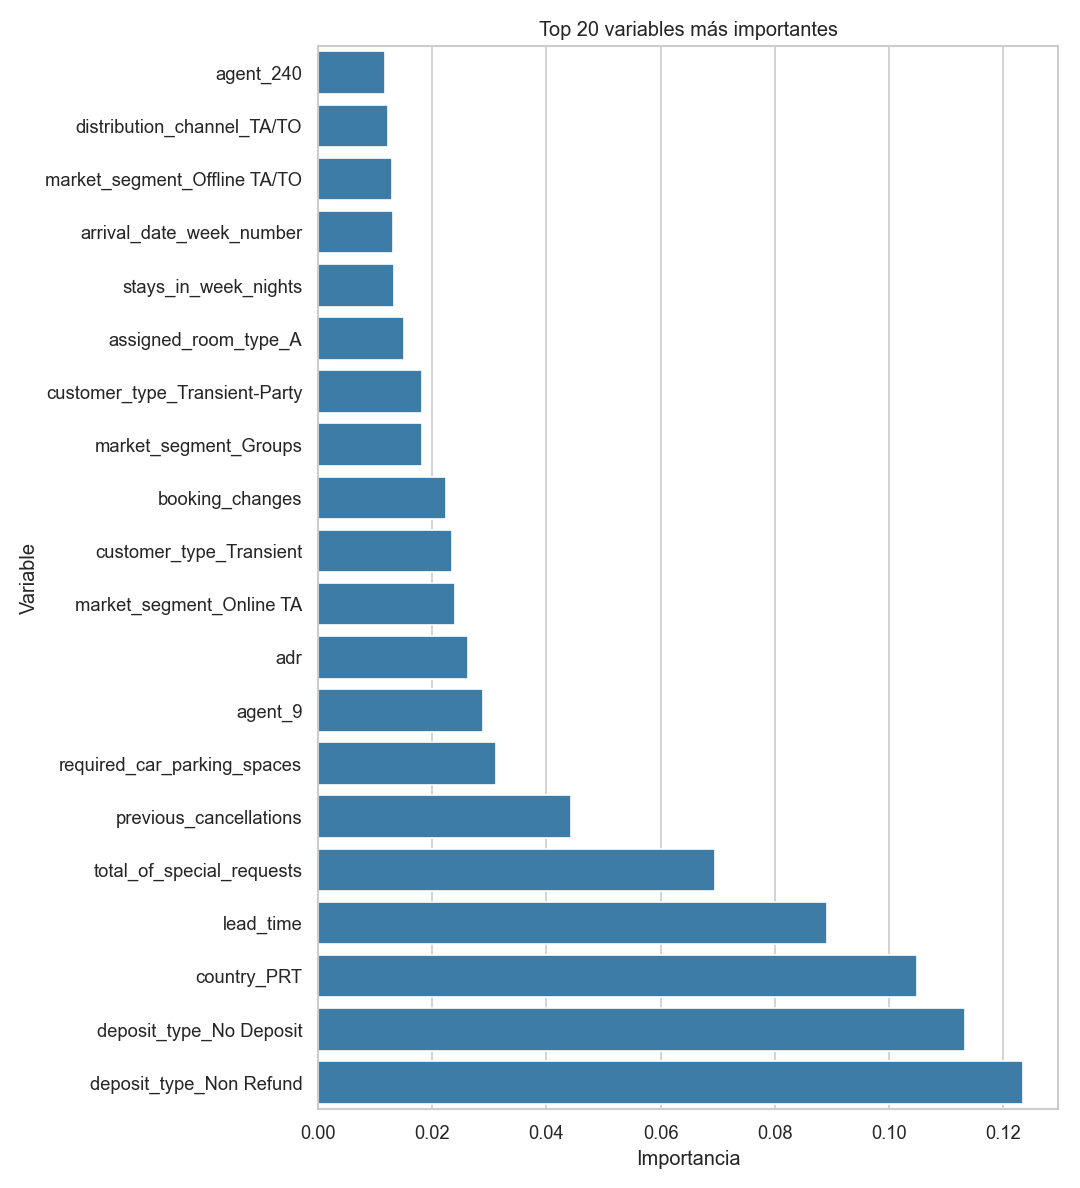
\includegraphics[width=\linewidth]{feature_importance.png}
    \caption{Importancia de variables del Random Forest: coincide en lo esencial con el
    \emph{ranking} SHAP del ganador (depósito, \var{lead\_time}, país, cancelaciones
    previas\dots).}
    \label{fig:fimp}
  \end{subfigure}
  \caption{Interpretabilidad global por dos familias de modelos: SHAP sobre el XGBoost
  ganador (a) y la importancia interna del Random Forest (b). Su coincidencia refuerza
  que el sistema aprende patrones reales, no artefactos de un algoritmo.}
  \label{fig:interp}
\end{figure*}

\paragraph{A nivel local.} SHAP también explica reservas individuales. La
Figura~\ref{fig:waterfall} desglosa una reserva de \textbf{altísimo riesgo}
($p\approx1$): partiendo del riesgo medio, el depósito no reembolsable ($+3.45$) y las
cancelaciones previas ($+2.87$) la empujan con fuerza hacia ``cancela'', mientras que
solo unos pocos factores tiran ligeramente en sentido contrario.
Este tipo de explicación es lo que permite \textbf{justificar al negocio} por qué una
reserva concreta se marca como dudosa.

\begin{figure}[tb]
  \centering
  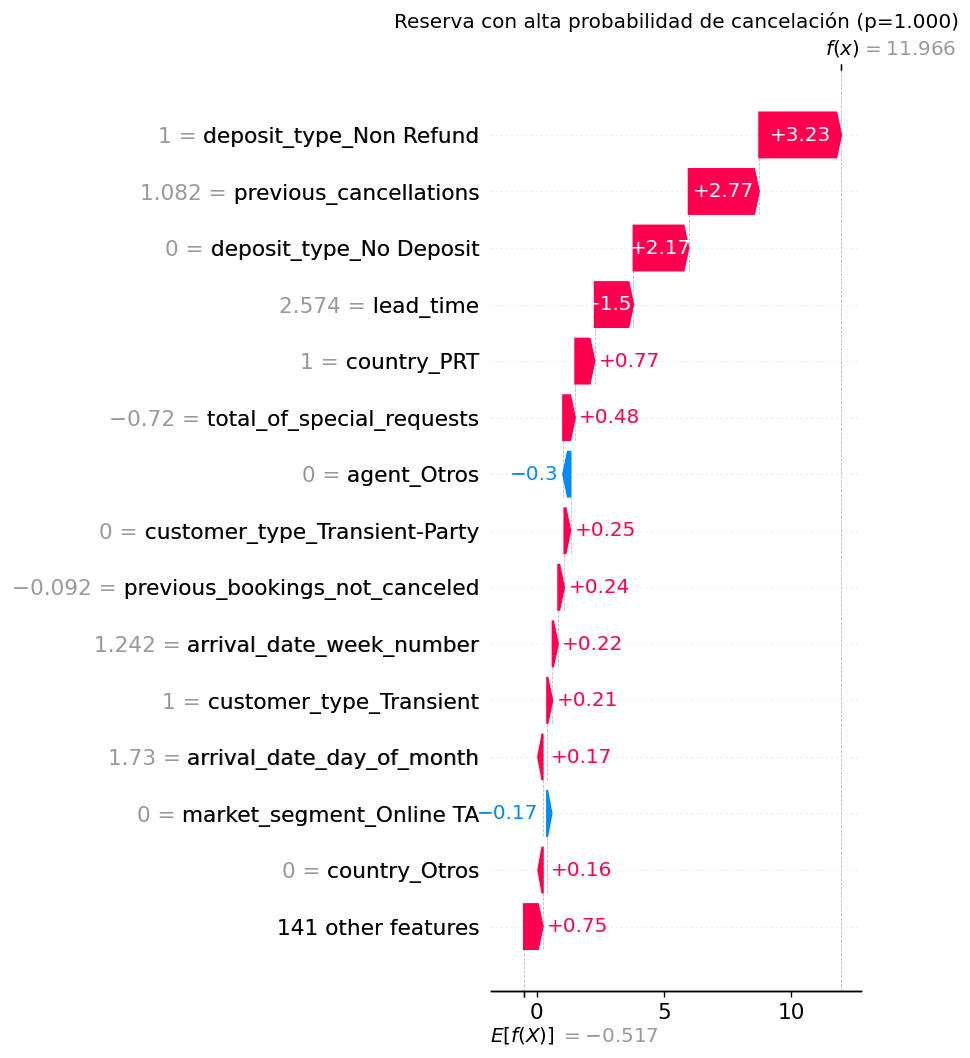
\includegraphics[width=\columnwidth]{shap_waterfall_ejemplo1.png}
  \caption{Explicación local (\emph{waterfall} SHAP) de una reserva de ejemplo con
  alta probabilidad de cancelación: contribución de cada variable a su predicción.}
  \label{fig:waterfall}
\end{figure}

% ============================================================================
\section{Resultados y elección final}

La evaluación se realiza sobre un \textbf{conjunto de prueba} de 23\,713 reservas
(20\,\% del total) que el modelo no usó al entrenar (Tabla~\ref{tab:resultados}). Las
cifras corresponden a los hiperparámetros ya optimizados.

\subsection{La métrica: ROC-AUC}

La métrica principal es el \textbf{ROC-AUC} (área bajo la curva ROC). En vez de medir
cuántas predicciones acierta con un umbral fijo, evalúa la capacidad del modelo de
\textbf{ordenar} las reservas por riesgo: equivale a la probabilidad de que, tomadas
al azar una reserva cancelada y otra no, el modelo asigne mayor riesgo a la cancelada.
Vale $0.5$ si no distingue mejor que el azar y $1$ si las ordena perfectamente. Se
eligió por tres razones alineadas con el caso de uso:

\begin{itemize}
  \item \textbf{Robusta al desbalance:} a diferencia de la \emph{accuracy}, no se
        deja engañar por la clase mayoritaria (un modelo que dijera ``nadie cancela''
        acertaría el 63\,\% pero sería inútil).
  \item \textbf{Independiente del umbral:} no fija de antemano a partir de qué
        probabilidad se considera ``cancelará'', de modo que el hotel puede mover ese
        punto de corte según su coste ---más agresivo para llenar plazas, más prudente
        si una falsa alarma es cara.
  \item \textbf{Comparable:} da una cifra única y homogénea para ordenar los cinco
        modelos.
\end{itemize}

Como el valor de negocio está precisamente en \emph{priorizar} reservas por riesgo
(para \emph{overbooking}, depósitos o retención), una métrica de \textbf{ordenación}
es la más adecuada. Se reportan además \emph{recall} y precisión por su lectura
directa para el negocio.

Formalmente, el ROC-AUC es el área bajo la curva que enfrenta la tasa de verdaderos
positivos $\mathrm{TPR}(\tau)$ frente a la de falsos positivos $\mathrm{FPR}(\tau)$ al
variar el umbral, $\mathrm{AUC} = \int_0^1 \mathrm{TPR}\bigl(\mathrm{FPR}^{-1}(u)\bigr)\,du$,
y equivale al estadístico de Mann--Whitney\,\textsuperscript{[1]}: si $X_1$ es el riesgo
predicho para una reserva cancelada al azar y $X_0$ el de una no cancelada,
\begin{equation}
\mathrm{AUC} = P(X_1 > X_0).
\end{equation}
Es decir, mide directamente la probabilidad de ordenar correctamente un par
cancelada/no-cancelada, independientemente del umbral.

\begin{table}[t]
  \centering
  \small
  \setlength{\tabcolsep}{4pt}
  \renewcommand{\arraystretch}{1.2}
  \begin{tabular}{@{}lccccc@{}}
    \toprule
    \textbf{Modelo} & Acc. & Prec. & Rec. & F1 & \textbf{ROC-AUC} \\
    \midrule
    \textbf{XGBoost} & 0.881 & 0.859 & 0.814 & 0.836 & \textbf{0.9529} \\
    Red neuronal     & 0.861 & 0.845 & 0.769 & 0.805 & 0.9353 \\
    Random Forest    & 0.856 & 0.872 & 0.720 & 0.789 & 0.9338 \\
    Árbol decisión   & 0.846 & 0.822 & 0.747 & 0.783 & 0.9235 \\
    Reg. logística   & 0.803 & 0.723 & 0.764 & 0.743 & 0.8862 \\
    \bottomrule
  \end{tabular}
  \caption{Métricas sobre el conjunto de prueba. XGBoost domina en la métrica
  principal (ROC-AUC) y en F1.}
  \label{tab:resultados}
\end{table}

\subsection{El modelo ganador}

\textbf{Se elige XGBoost} (ROC-AUC $=0.9529$). Supera al resto en la métrica principal
y en F1, y aun así entrena en pocos segundos. En términos de negocio, con el umbral
por defecto detecta el \textbf{81\,\% de las cancelaciones reales} (\emph{recall}
$0.81$) con una \textbf{precisión del 86\,\%}: un buen equilibrio para actuar sin
generar demasiadas falsas alarmas. El Random Forest es el más conservador (más
precisión, menos \emph{recall}), preferible si una falsa alarma fuese muy costosa. Las
curvas ROC (Figura~\ref{fig:roc}) confirman esta jerarquía.

\begin{figure}[tb]
  \centering
  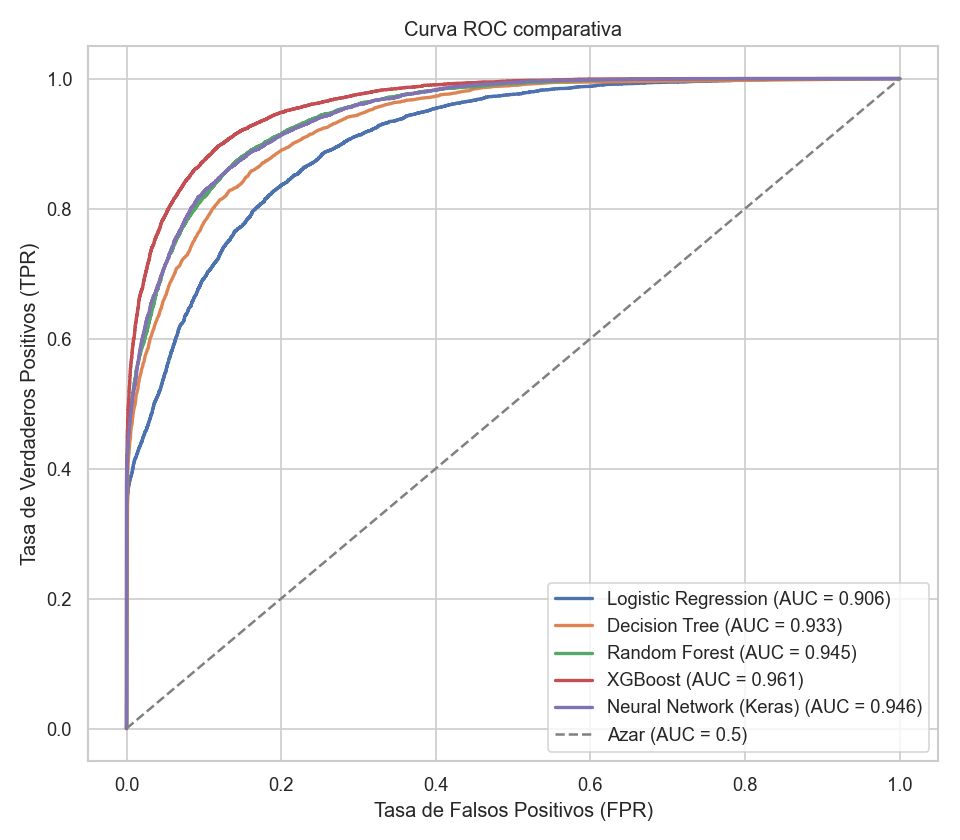
\includegraphics[width=\columnwidth]{roc_curves.png}
  \caption{Curvas ROC comparativas. Cuanto más cerca de la esquina superior
  izquierda, mejor; XGBoost domina al resto.}
  \label{fig:roc}
\end{figure}

Su ventaja teórica está en cómo optimiza: en cada iteración $t$ aproxima la pérdida con
una expansión de Taylor de segundo orden y penaliza la complejidad del árbol,
minimizando el objetivo regularizado de Chen y Guestrin\,\textsuperscript{[2]}
\begin{equation}
\mathcal{L}^{(t)} \approx \sum_{i=1}^{n}
  \Bigl[ g_i\,f_t(\mathbf{x}_i) + \tfrac{1}{2} h_i\,f_t^{2}(\mathbf{x}_i) \Bigr]
  + \gamma T + \tfrac{1}{2}\lambda \sum_{j=1}^{T} w_j^{2},
\end{equation}
donde $g_i$ y $h_i$ son los gradientes de primer y segundo orden de la pérdida en la
predicción previa, $T$ es el número de hojas, $w_j$ sus pesos y $\gamma,\lambda$
regularizadores. Esta penalización explícita de la complejidad explica su robustez y
eficiencia en CPU.

La matriz de confusión del ganador (Figura~\ref{fig:cm}) desglosa su comportamiento
sobre las 23\,713 reservas de prueba: detecta \textbf{7193} de las 8835 cancelaciones
reales y se le escapan 1642 (los falsos negativos), generando solo \textbf{1178}
falsas alarmas sobre las reservas que no se cancelaban.

\begin{figure}[tb]
  \centering
  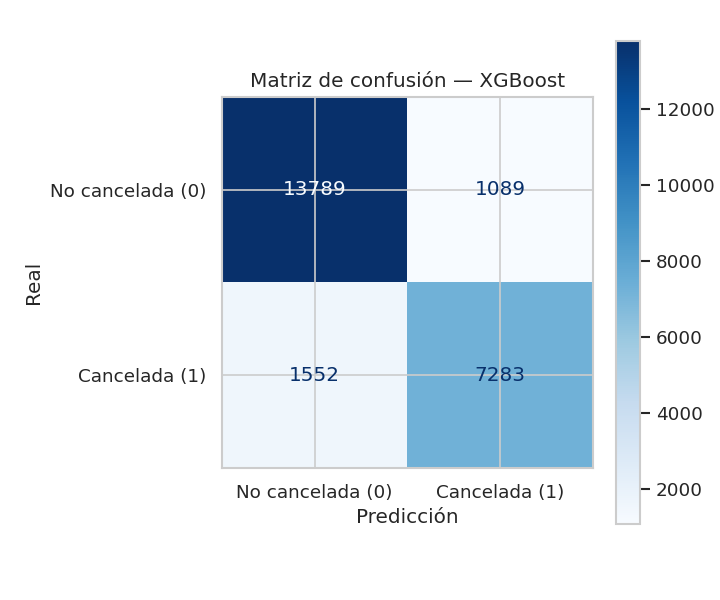
\includegraphics[width=0.86\columnwidth]{confusion_matrix_best.png}
  \caption{Matriz de confusión del modelo ganador (XGBoost) sobre el conjunto de
  prueba: los aciertos están en la diagonal.}
  \label{fig:cm}
\end{figure}

% ============================================================================
\section{Reflexión crítica: limitaciones y mejoras}

\textbf{Limitaciones actuales.}
\begin{itemize}
  \item \textbf{Validación temporal pendiente:} la partición es aleatoria. Como las
        reservas tienen fecha (2015--2017), una división \emph{por tiempo}
        (entrenar con el pasado, probar con el futuro) sería más realista y
        probablemente daría una cifra algo más baja, pero más fiable.
  \item \textbf{Desbalance sin tratamiento explícito:} se aborda con estratificación y
        una métrica adecuada, no con técnicas de reequilibrado. El balanceo
        (\var{class\_weight}, SMOTE) se exploró y sube el \emph{recall} a costa de
        precisión, pero deja el ROC-AUC casi igual, por lo que no se incorpora al
        \emph{pipeline} de producción.
  \item \textbf{Cardinalidad simplificada:} agrupar las categorías raras en
        \var{Otros} sacrifica parte de su información individual.
  \item \textbf{Umbral fijo en 0.5:} no se ha ajustado a un objetivo de negocio
        concreto.
\end{itemize}

\textbf{Líneas de mejora.}
\begin{itemize}
  \item \textbf{Un modelo por hotel.} El EDA mostró que el \emph{City Hotel} y el
        \emph{Resort Hotel} se comportan casi como dos negocios distintos, con
        estacionalidad y tasa de cancelación diferentes. Entrenar un modelo
        especializado para cada uno, en lugar de uno único, podría capturar mejor sus
        patrones propios, a costa de mantener y servir dos modelos.
  \item \textbf{Validación temporal} para cifras más fiables que la partición
        aleatoria.
  \item \textbf{\emph{Embeddings}} para las categóricas de alta cardinalidad
        (\var{country}, \var{agent}), que preservarían más señal que el agrupamiento.
  \item \textbf{Infraestructura con más memoria} (p.\,ej. Hugging Face Spaces) para
        reactivar la carga del modelo desde el \emph{Model Registry} de MLflow en el
        despliegue público, hoy limitado por la RAM del \emph{tier} gratuito.
\end{itemize}

% ============================================================================
\section{Conclusiones}

Este trabajo ha abordado la predicción de cancelaciones de reservas hoteleras como un
problema de clasificación binaria de principio a fin: desde un análisis exploratorio que
\textbf{detecta y corrige fugas de información} ---el origen del optimismo de versiones
previas--- hasta un sistema desplegado en producción. La decisión metodológica más
relevante fue \emph{anteponer la honestidad al número}: eliminar las variables de
\emph{check-in} (\var{required\_car\_parking\_spaces}, \var{assigned\_room\_type}) rebaja
el ROC-AUC de un $0.9614$ engañoso a un \textbf{$0.9529$ realista}, una cifra que sí
mide lo que el modelo podrá hacer ante una reserva futura.

De las cinco familias comparadas en igualdad de condiciones, \textbf{XGBoost} resulta la
ganadora, combinando la mejor métrica de ordenación con un coste de entrenamiento mínimo.
Un componente relevante del \emph{pipeline} es el \texttt{RareCategoryGrouper}, un
transformador propio ---no disponible en \texttt{scikit-learn}--- que aplica una reducción
supervisada de cardinalidad: ajustado solo en entrenamiento, conserva las categorías con
señal de cancelación extrema en \var{country}, \var{agent} y \var{company} y agrupa el resto,
reduciendo de 902 a 144 columnas sin pérdida de poder predictivo. Junto con las variables
derivadas de la ausencia informativa (\var{has\_company}/\var{has\_agent}), preserva la mayor
parte de la señal. La interpretabilidad con SHAP confirma, además, que el modelo se apoya en
factores con sentido de negocio (depósito no reembolsable, país, antelación, cancelaciones
previas), no en artefactos.

El resultado es un sistema reproducible y \textbf{accesible en línea} (API REST, interfaz
web y registro de experimentos), que no solo predice sino que \emph{explica} cada decisión.
Entre las líneas de mejora, la más respaldada por el análisis es \textbf{separar el sistema
en dos modelos especializados}, uno por tipo de hotel (\emph{City} y \emph{Resort}): el EDA
mostró que se comportan como negocios distintos, con estacionalidad y tasa de cancelación
propias, por lo que un modelo por hotel capturaría mejor sus patrones. Otras vías
---validación temporal o \emph{embeddings} para la alta cardinalidad--- complementan ese
camino más allá del alcance de esta memoria.

% ============================================================================
\section*{Bibliografía}
\small
\begin{enumerate}[label={[\arabic*]}, leftmargin=2.2em]
  \item \emph{Receiver operating characteristic} (curva ROC, AUC y su equivalencia con
        el estadístico de Mann--Whitney). Wikipedia (consultado en junio de 2026).
        \url{https://en.wikipedia.org/wiki/Receiver_operating_characteristic}
  \item T. Chen y C. Guestrin. \emph{XGBoost: A Scalable Tree Boosting System}.
        Proceedings of the 22nd ACM SIGKDD, 2016.
        \url{https://doi.org/10.1145/2939672.2939785}
  \item S. M. Lundberg y S.-I. Lee. \emph{A Unified Approach to Interpreting Model
        Predictions}. Advances in Neural Information Processing Systems (NeurIPS), 2017.
  \item N. Antonio, A. de Almeida y L. Nunes. \emph{Hotel booking demand datasets}.
        Data in Brief, vol.\ 22, 2019. \url{https://doi.org/10.1016/j.dib.2018.11.126}
\end{enumerate}

\end{document}
